Die Auswertung kann auf zwei Arten passieren. Die einfache Variante, die bei den Vorversuchen genutzt wird, ist mit den eigenen Augen die Grösse und Verteilung des Rots auf dem Tape ab zu schätzten.

Um dieses Gefühl zu quantivizieren wurde eine Pipeline zur digitalen Auswertung entwickelt. In einem ersten Schritt, illustiert in \ref{fig:Bildverarbeitnugskonzpet}, wird das Tape in der Fotografie ausgewählt, dann in ein schwarz weiss Bild übersetzt. Der zweite Schritt kann in dem Bild die Farbflecken erkennen. Um aus dem Bild quantitative Zahlen zu bekommen, werden die Farbflecken einzeln erkannt und in die Datenback gespeichert. In der Datenbank können dann statistische Aussagen wie die Verteilung und der relative Flächenanteil gemacht werden.

\begin{figure}
    \centering
    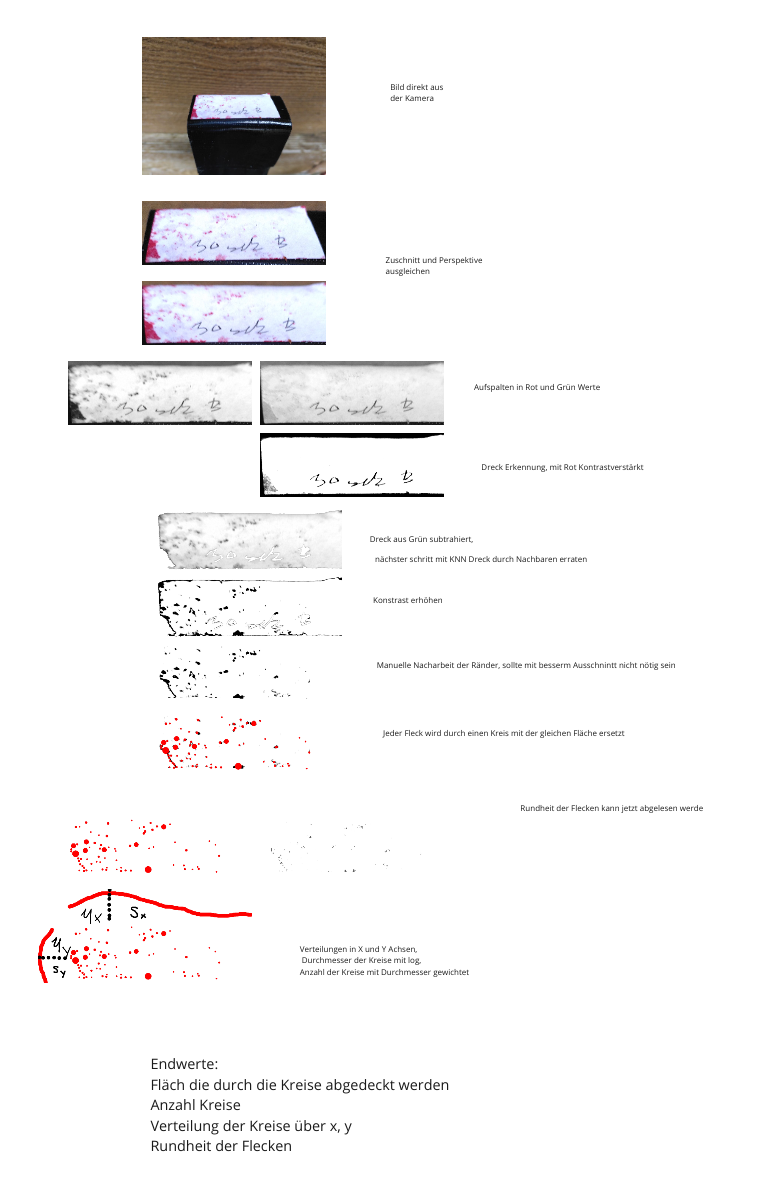
\includegraphics[width=0.8\textwidth]{Bilder/Screenshotfrom2024-04-0112-59-42.png}
    \caption{Bildverarbeitung Konzept}
    \label{fig:Bildverarbeitnugskonzpet}
\end{figure}

\newpage
